\documentclass[11pt]{article}
\usepackage[margin=1.15in]{geometry}
\usepackage{amsmath,amssymb,amsthm}
\usepackage{graphicx}
\usepackage{booktabs}
\usepackage{xcolor}
\usepackage[colorlinks=true,linkcolor=blue!60!black,citecolor=blue!60!black,urlcolor=blue!60!black]{hyperref}

\newtheoremstyle{itheads}{\topsep}{\topsep}{}{}{\itshape}{.}{.5em}{}
\theoremstyle{itheads}
\newtheorem{theorem}{Theorem}
\newtheorem{proposition}{Proposition}
\newtheorem{lemma}{Lemma}
\newtheorem{corollary}{Corollary}

\newcommand{\E}{\mathbb{E}}
\newcommand{\R}{\mathbb{R}}
\newcommand{\sech}{\operatorname{sech}}
\newcommand{\artanh}{\operatorname{artanh}}

\title{When the Grass Is Greener\\[4pt]
{\large Three-Shot Search on an Exponentiated Ornstein--Uhlenbeck Landscape}}
\author{Peter Cotton}
\date{\normalsize First version: April 6, 2022. This version: September 3, 2026.}

\begin{document}
\maketitle

\begin{abstract}
\noindent A searcher evaluates a random landscape at three points, one at a
time, and is paid the value at the final point. The landscape is the
exponential of a stationary Ornstein--Uhlenbeck path. We solve the
problem exactly. With two evaluations the optimal rule has three
regimes: abandon a below-average start, keep an exceptional one, and
otherwise step a distance given in closed form. With three
evaluations the question is where to commit after observing values
$b$ and $d$ at bracket correlation $\rho$. For $b=d$, every interior
point of the bracket has the same conditional mean as some exterior
point, and conditional variance larger by the constant factor
$(1+\rho)/(1-\rho)=e^{2\Theta}$. The interior problem reduces to a
parabola on an interval. The best interior point beats every
alternative exactly when $b$ lies between a quadratic root and
$e^{2\Theta}$. The optimal interior point is the midpoint for
moderate $b$; it splits into a pair that moves toward the ends as
$b$ grows, and reaches them at $b=e^{2\Theta}$, above which the
searcher should stay at an observed point. The interior option
raises expected value by about one percent at most. We verify the
landscape assumption on 77{,}040 WiFi measurements and interpret the
three evaluations as an incumbent strategy, one pivot, and a
commitment.
\end{abstract}

\section{Introduction}

How many pivots does a firm get? In randomized trials, about three
quarters of startups did not pivot at all over a year, about a fifth
pivoted once, and fewer than one in ten pivoted more than once
(Camuffo et al.\ 2020, 2024). Training founders to search more
scientifically raised the frequency of a single pivot and lowered
the frequency of repeated pivots. In practice, strategic search
involves very few evaluations.

Callander (2011) modeled this kind of search as trial and error on
an unknown function drawn from a Brownian motion. Each trial is
implemented and its outcome observed. Most work in this tradition
assumes myopic agents. Bardhi and Callander (2026) list farsighted
search with a free choice of location as an open problem.

We solve the smallest such problem exactly. The landscape is the
exponential of a stationary Ornstein--Uhlenbeck path. Mean reversion
means that performance far from known territory regresses to the
industry average. The exponential means that small differences in
fit produce large differences in sales, so an untried strategy has
extra value on average.

The searcher knows the performance of an incumbent strategy. She may
try one more. Then she must commit. With two evaluations the optimal
rule is a threshold rule: abandon a below-average incumbent, keep an
exceptional one, and otherwise step a distance that we give in
closed form. With three evaluations the question is where to commit
after the trial: between the two known strategies, beyond the better
one, or at one of them. We compute the answer exactly. Commitment
between the two is optimal when both values are good but not
exceptional. The commitment point is the midpoint for moderate
values and moves toward the better-known end as the values improve.
Above an exact ceiling the searcher should stay where she is.

The interior option is worth about one percent of expected value at
the optimum. Most of the value of the final pivot comes from the
information it produces. On landscapes that decorrelate quickly, it
is better to probe far away, and the formulas say so: the interior
premium is first order in the bracket correlation. We check the
landscape assumption on 77{,}040 WiFi measurements across a
university floor. The detrended log signal is Gaussian and its
spatial correlation is exponential with $R^2=0.98$. A replay on
that data matches the ranking of policies that the formulas predict
(Section~\ref{sec:wifi}).

\section{Related work}

Callander (2008) introduced the Brownian policy landscape. In that
paper, delegation to a biased expert survives only when the bias is
below $\sigma^{2}/2\mu$. The 2011 papers use the landscape for
search. An agent experiments when the incumbent outcome is worse
than $\alpha=\sigma^{2}/2|\mu|$ and stops otherwise. Search ends
almost surely, often at a mediocre policy. Simulated runs change
policy between one and four times, which is consistent with the
pivot counts above. Later papers derive similar thresholds for
precedent (Callander and Clark 2017), agenda control (Callander and
McCarty 2024), and risk-averse learning (Callander and Matouschek
2019). In all of these the number of evaluations is endogenous and
payoffs accrue every period. In our problem the number of
evaluations is fixed at three, only the final placement is paid, and
the landscape mean-reverts.

Callander and Hummel (2014) analyze a two-period game in which each
of two policymakers can experiment once. The equilibrium has two
exact cutoffs, and the first mover sometimes experiments although
the status quo already delivers his ideal outcome. The players are
strategic and payoffs accrue in both periods. Ganz (2020) studies an
organization that allows a manager one offline trial before an
online choice. That is a two-evaluation problem in which only the
second evaluation is paid, and some of its boundaries are computed
numerically. We solve the three-evaluation single-agent problem in
closed form.

Other papers obtain farsighted results under other restrictions.
Urgun and Yariv (2025) require search to be contiguous; the searcher
chooses speed and stops at a closed-form drawdown. Cetemen, Urgun
and Yariv (2023) extend this to teams and Wong (2025) to flow
payoffs. Bardhi (2024) chooses $k$ sample locations at once to
estimate a project. Garfagnini and Strulovici (2016), Carnehl and
Schneider (2025), and Callander, Lambert and Matouschek
(forthcoming) study infinite sequences of short-lived agents. Aybas
and Callander (2025) allow Ito diffusion landscapes, including the
Ornstein--Uhlenbeck case, in a one-shot cheap-talk game. That is the
only mean-reverting landscape we know of in this literature. Bardhi
(2024) also proves that the OU kernel is the only powered-exponential
covariance with the Markov property, which supports our choice of
landscape.

In the optimization literature the same object appears with large
budgets. Calvin (1997) derives average-case convergence rates under
Wiener measure. Grill, Valko and Munos (2018) approximate the
maximum of a Brownian path. Grosse, Zhang and Hennig (2023) extend
this to Gaussian-process samples and prove regret rates. Alabert and
Caballero (2018) compute the law of the minimum of a conditioned
bridge in order to compare fixed sampling designs. Malladi (2025)
and Banchio and Malladi (2025) solve worst-case versions with no
prior and a Lipschitz bound in place of volatility. Hodgson and
Lewis (2025) estimate a Gaussian-process search model on clickstream
data and solve the policy numerically. We are not aware of a
closed-form solution for a small fixed budget of adaptive
evaluations under a Bayesian prior.

Glick and Myers (2015) tested the one-evaluation problem on lab
subjects. Subjects respond to the Brownian structure but modify too
much when the variance is high.

\section{The model: three evaluations of an exponentiated OU path}

Let $X$ be a stationary Ornstein--Uhlenbeck process on $\R$ with
$\E[X_t]=0$, unit marginal variance, and covariance kernel
\begin{equation}
k(s,t) \;=\; e^{-\kappa|s-t|}.
\end{equation}
The landscape is $f(t)=\exp(X_t)$: locally continuous, mean-reverting in
its logarithm, with occasional high peaks where excursions are magnified
by the exponential. A searcher samples $f$ at a first location, which we
take to be $t_0=0$ by translation invariance, discovering $X_0=b$. Two
further evaluations at locations $t_1$ and then $t_2$ follow, each
chosen with knowledge of all values so far, and the payoff is the value
at the final location, $u=\E\left[f(t_2)\right]$. Conditional on the
observations gathered by the time $t_2$ is chosen, $X_{t_2}$ is
Gaussian with some mean $\mu$ and variance $\nu$, and
\begin{equation}\label{eq:lognormal}
\log \E\!\left[e^{X_{t_2}}\,\middle|\,\mathcal{F}\right]
\;=\; \mu + \tfrac{1}{2}\nu ,
\end{equation}
where $\mathcal{F}$ denotes the observed locations and values. (The
unconditional distribution after adaptive placement need not be
Gaussian; every use of \eqref{eq:lognormal} below is conditional.) The
searcher is thus paid for conditional mean and conditional variance in
equal measure: a final location with residual uncertainty carries a
lognormal bonus of half its variance.

Figure~\ref{fig:problem} shows the decision this paper solves.
Two conventions tidy the boundary cases. A searcher may take a location
to infinity, which by mean reversion is equivalent to sampling a fresh
$N(0,1)$ value independent of everything seen; and a searcher may
finish at an observed location, receiving its known value. Neither
changes the substance of any result.

\begin{figure}[t]
\centering
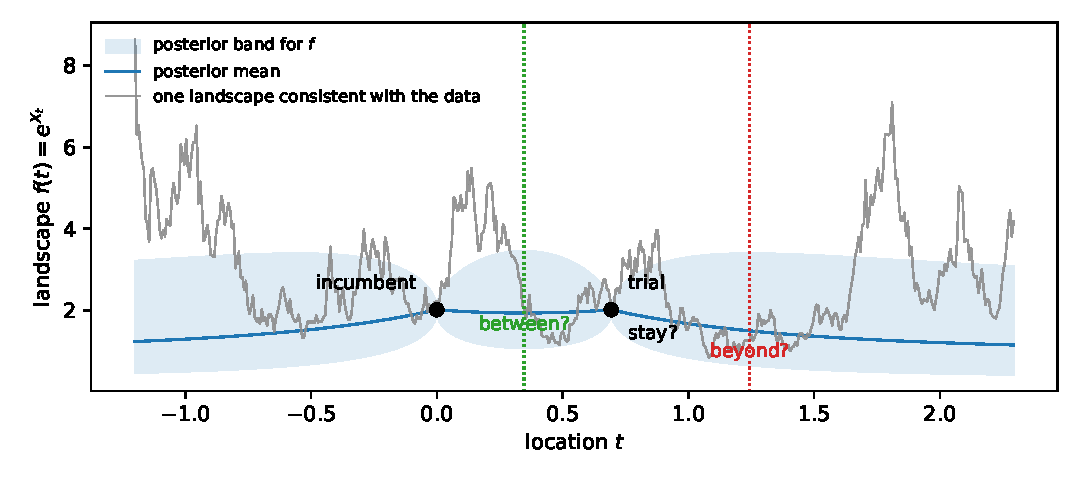
\includegraphics[width=0.92\textwidth]{figures/problem.pdf}
\caption{The problem. Two locations have been evaluated and returned
equal values (dots); the shaded region is the posterior band for the
landscape and the grey curve one landscape consistent with the data.
The final evaluation is the consequential one: settle between the
anchors, step out past an end, or stay at an observed point. The
paper computes which, exactly, as a function of the anchor value and
the bracket correlation.}
\label{fig:problem}
\end{figure}

\section{Two evaluations: flee, explore, or stay}

Given only $X_0=b$, a candidate second location at distance $t$ has
$X_t \sim N\!\left(b\lambda,\,1-\lambda^{2}\right)$ with
$\lambda=e^{-\kappa t}\in(0,1]$. From \eqref{eq:lognormal},
\begin{equation}
\log \E\!\left[e^{X_t}\,\middle|\,X_0=b\right]
\;=\; b\lambda + \tfrac{1}{2}\!\left(1-\lambda^{2}\right)
\;=\; -\tfrac{1}{2}\left(\lambda-b\right)^{2} + \tfrac{1}{2}\left(b^{2}+1\right),
\end{equation}
maximized over $\lambda\in[0,1]$ at $\lambda^{*}=\min\{\max\{b,0\},1\}$.

\begin{proposition}[Two-shot policy]\label{prop:twoshot}
The optimal second location and its log-value $\zeta(b)$ are
\begin{equation}
t^{*} \;=\;
\begin{cases}
\infty & b<0 \quad(\text{flee}),\\[2pt]
-\tfrac{1}{\kappa}\log b & 0\le b\le 1 \quad(\text{explore}),\\[2pt]
0 & b>1 \quad(\text{stay}),
\end{cases}
\qquad
\zeta(b) \;=\;
\begin{cases}
\tfrac{1}{2} & b<0,\\[2pt]
\tfrac{1}{2}\left(b^{2}+1\right) & 0\le b\le 1,\\[2pt]
b & b>1 .
\end{cases}
\end{equation}
\end{proposition}

A below-median first value is abandoned, and an exceptional one is
kept: already at two shots, an observed location can be the optimal
final location. Practitioners know this fork as pivot or persevere
(Ries 2011); the proposition supplies its thresholds and the size of
the step when pivoting wins. In between, the searcher steps to the distance at which the
prior pull toward the mean exactly balances the anchor's height. The
value $\zeta$ serves as the exterior benchmark throughout: by the
Markov property, any placement beyond all existing observations faces a
fresh copy of this problem anchored at the nearest observation.

\section{Bridge moments, and what composes how}

Suppose values $X_0=b$ and $X_{t_1}=d$ are known, with bracket
correlation $\rho=e^{-\kappa t_1}$ and rapidity
$\Theta=\artanh\rho$. For an interior location let
$\lambda_2=e^{-\kappa t_2}$ and $\lambda=e^{-\kappa(t_1-t_2)}$ be the
correlations to the two ends, $\lambda_2\lambda=\rho$, with rapidities
$\theta_2=\artanh\lambda_2$ and $\theta=\artanh\lambda$. Gaussian
conditioning gives the bridge moments
\begin{equation}\label{eq:bridge}
\mu \;=\; \frac{\lambda_2\!\left(1-\lambda^{2}\right)b
+ \lambda\!\left(1-\lambda_2^{2}\right)d}{1-\rho^{2}},
\qquad
\nu \;=\; \frac{\left(1-\lambda_2^{2}\right)\left(1-\lambda^{2}\right)}
{1-\rho^{2}} .
\end{equation}
For $b=d>0$ the bridge sags: the mean is below $b$ everywhere
strictly inside, pulled toward the process mean, while the variance
rises from zero at the ends to a maximum at the middle.

A caution on what is additive. Correlations across consecutive
intervals multiply, $\rho(t+s)=\rho(t)\,\rho(s)$, so the additive
coordinate for composing intervals is $\kappa t=-\log\rho$, not the
rapidity. The rapidity earns its keep through a different identity:
for equal anchors $d=b$ the bridge mean is
\begin{equation}\label{eq:meanadd}
\mu \;=\; b\,\frac{\lambda_2+\lambda}{1+\lambda_2\lambda}
\;=\; b\tanh\!\left(\theta_2+\theta\right),
\end{equation}
which matches the mean of the exterior point at correlation
$\tanh(\theta_2+\theta)$ to its anchor. This is a mean-matching device
we use next, not a composition law. The bridge variance also takes a
hyperbolic product form: substituting $1-\tanh^{2}=\sech^{2}$ into
\eqref{eq:bridge},
\begin{equation}\label{eq:varprod}
\nu \;=\; \sech\!\left(\theta_2+\theta\right)
\sech\!\left(\theta_2-\theta\right),
\end{equation}
while an exterior point at correlation $\lambda'=\tanh\theta'$ to its
anchor has variance $1-\tanh^{2}\theta'=\sech^{2}\theta'$.

\section{Matched-mean dominance at a constant variance ratio}

\begin{theorem}[Bridge dominance, equal anchors]\label{thm:dominance}
Let $d=b$ and let $t_2\in(0,t_1)$ be an interior location with
rapidities $(\theta_2,\theta)$. The exterior location at composed
rapidity $\theta'=\theta_2+\theta$ has the same conditional mean
$b\tanh(\theta_2+\theta)$, and the ratio of conditional variances is
the same at every interior point:
\begin{equation}\label{eq:constratio}
\frac{\nu_{\mathrm{inside}}}{\nu_{\mathrm{outside}}}
\;=\; \frac{\cosh(\theta_2+\theta)}{\cosh(\theta_2-\theta)}
\;=\; \frac{1+\tanh\theta_2\tanh\theta}{1-\tanh\theta_2\tanh\theta}
\;=\; \frac{1+\rho}{1-\rho} \;=\; e^{2\Theta} \;>\; 1 .
\end{equation}
Consequently the interior point's conditional distribution dominates
its mean-matched exterior rival in the Gaussian convex order, and its
expected payoff is at least as large for every convex payoff with
finite expectation, strictly so for the exponential.
\end{theorem}

\begin{proof}
The mean statement is \eqref{eq:meanadd}. The ratio of
\eqref{eq:varprod} to $\sech^{2}(\theta_2+\theta)$ is
$\cosh(\theta_2+\theta)/\cosh(\theta_2-\theta)$, and expanding both
via $\cosh(A\pm B)=\cosh A\cosh B\pm\sinh A\sinh B$ gives
$(1+\tanh\theta_2\tanh\theta)/(1-\tanh\theta_2\tanh\theta)$, which is
$(1+\rho)/(1-\rho)$ because $\tanh\theta_2\tanh\theta
=\lambda_2\lambda=\rho$ on the bracket. Two Gaussians with equal
means and ordered variances are ordered in the convex order (the
wider equals the narrower plus independent noise), and
\eqref{eq:lognormal} is the exponential case.
\end{proof}

The amplification is a property of the bracket, not the position:
threefold at $\rho=\tfrac12$, nineteenfold at $\rho=0.9$, unbounded as
$\rho\uparrow 1$. At the bracket's ends both variances vanish; their
ratio still tends to $e^{2\Theta}$. Dominance over mean-matched
exterior rivals, which the theorem explicitly constructs, decides
nothing by itself: the exterior player may choose any
correlation, and an observed anchor may simply be kept. The object
that can fail to exist is different: an \emph{unvisited} point whose
conditional mean matches the best \emph{observed} value. Mean
reversion caps unvisited conditional means strictly below a high
anchor, and whether the variance bonus makes up the shortfall is
precisely the question the phase diagram answers. The next section
makes this exact.

\section{The constrained parabola and the complete symmetric solution}

Parametrize the interior by $x=\lambda_2\in(\rho,1)$ and set
\begin{equation}\label{eq:mdef}
C \;=\; \frac{1+\rho}{1-\rho}\;=\;e^{2\Theta},
\qquad
m \;=\; \frac{x+\rho/x}{1+\rho}
\;\in\;\left[\frac{2\sqrt{\rho}}{1+\rho},\,1\right),
\end{equation}
under which mirror points $x\leftrightarrow\rho/x$ coincide, the lower
endpoint of $m$ is the bracket middle, and, using
$\left(1-x^{2}\right)\left(1-\rho^{2}/x^{2}\right)
=\left(1+\rho\right)^{2}\left(1-m^{2}\right)$, the equal-anchor
interior log-utility becomes a constrained parabola:
\begin{equation}\label{eq:parabola}
L_{\mathrm{inside}}(m) \;=\; b\,m + \frac{C}{2}\left(1-m^{2}\right),
\qquad
m^{*} \;=\; \operatorname{clip}\!\left(\frac{b}{C};\;
\frac{2\sqrt{\rho}}{1+\rho},\,1\right).
\end{equation}
This is the organizing object of the paper: the entire symmetric
analysis reads off the position of the unconstrained peak $b/C$
relative to the interval.

\begin{theorem}[Pitchfork]\label{thm:pitchfork}
The bracket middle is the interior optimum iff
$b/C\le 2\sqrt{\rho}/(1+\rho)$, i.e.
\begin{equation}
b \;\le\; \frac{2\sqrt{\rho}}{1-\rho} \;=\; \sinh 2\tau,
\qquad \tau=\artanh\sqrt{\rho}.
\end{equation}
For $\sinh 2\tau<b<e^{2\Theta}$ the peak is interior and attained by
the mirror pair
\begin{equation}\label{eq:offmid}
x_{\pm} \;=\; \frac{b\left(1-\rho\right)
\pm\sqrt{b^{2}\left(1-\rho\right)^{2}-4\rho}}{2},
\qquad x_{+}x_{-}=\rho,
\end{equation}
with optimal value
\begin{equation}\label{eq:uoff}
U_{\mathrm{off}} \;=\; \frac{C}{2}+\frac{b^{2}}{2C}
\;=\;\tfrac12\!\left(b^{2}e^{-2\Theta}+e^{2\Theta}\right).
\end{equation}
For $b\ge e^{2\Theta}$ the peak $b/C\ge 1$ lies at or beyond the
interval's open end: $L_{\mathrm{inside}}$ is increasing in $m$, no
interior maximum is attained, and the interior supremum is the end
limit $b$.
\end{theorem}

\begin{proof}
$dL/dm=b-Cm$ vanishes at $m=b/C$; the interval endpoints translate
via \eqref{eq:mdef} into the stated $b$-thresholds
($b/C=2\sqrt{\rho}/(1+\rho)$ is $b=2\sqrt{\rho}/(1-\rho)$, and
$b/C=1$ is $b=(1+\rho)/(1-\rho)$; the hyperbolic forms follow from
$\tanh\tau=\sqrt{\rho}$). Solving $x+\rho/x=(1+\rho)\,b/C
=b\left(1-\rho\right)$ gives \eqref{eq:offmid}, and substituting
$m=b/C$ into \eqref{eq:parabola} gives \eqref{eq:uoff}.
\end{proof}

\begin{theorem}[Symmetric phase diagram]\label{thm:boundary}
For $d=b\ge 0$ the best interior point strictly beats every
alternative --- exterior placements and observed anchors alike ---
precisely for
\begin{equation}\label{eq:region}
b_{-}(\rho) \;<\; b \;<\; e^{2\Theta},
\qquad
b_{-}(\rho)=\frac{\sqrt{\rho}\left(2-\sqrt{2\left(1-\rho\right)}\right)}{1+\rho},
\end{equation}
the lower edge being the smaller root of
$b^{2}\left(1+\rho\right)-4b\sqrt{\rho}+2\rho=0$. For
$b\ge e^{2\Theta}$ the optimal final location is an \emph{observed}
one: staying at an anchor beats every unvisited point, interior or
exterior.
\end{theorem}

\begin{proof}
If $b\ge e^{2\Theta}$, Theorem~\ref{thm:pitchfork} gives interior
supremum $b$, unattained, while every exterior point loses to the
anchor pointwise: for $b>1$ and any $\lambda\in[0,1)$,
\begin{equation}
b-\left[b\lambda+\tfrac12\left(1-\lambda^{2}\right)\right]
\;=\;\left(1-\lambda\right)\!\left[b-\tfrac{1+\lambda}{2}\right]
\;>\;0
\end{equation}
(the suprema coincide at $b$; the dominance is strict at every
unvisited point): staying at an anchor wins. If $\sinh 2\tau<b<e^{2\Theta}$ the interior optimum
is $U_{\mathrm{off}}$, and both comparisons are one line: for $b>1$,
\begin{equation}
U_{\mathrm{off}} - b \;=\;
\tfrac12\,e^{-2\Theta}\!\left(b-e^{2\Theta}\right)^{2} \;>\;0,
\end{equation}
the arithmetic--geometric mean inequality applied to the two terms of
\eqref{eq:uoff}, with equality only at the tangency $b=e^{2\Theta}$
defining the upper edge; for $b\le 1$,
\begin{equation}
U_{\mathrm{off}} - \tfrac12\!\left(b^{2}+1\right) \;=\;
\tfrac12\!\left(e^{2\Theta}-1\right)\!\left(1-b^{2}e^{-2\Theta}\right)
\;>\;0 .
\end{equation}
If $b\le\sinh 2\tau$ the optimum is the middle, with value
$U_{\mathrm{mid}}=b\,\tfrac{2\sqrt{\rho}}{1+\rho}
+\tfrac{1-\rho}{2\left(1+\rho\right)}$; for $b\le 1$,
$U_{\mathrm{mid}}>\zeta(b)$ is the stated quadratic, and
$b_{-}\le 2\sqrt{\rho}/\left(1+\rho\right)<\sinh 2\tau$ places the
lower edge inside this regime. No gap opens above the middle regime:
when $\sinh 2\tau\le 1$ (i.e.\ $\rho\le 3-2\sqrt{2}$), the larger
quadratic root satisfies $b_{+}\ge\sinh 2\tau$, equivalent to
$\left(1-\rho\right)^{3}\ge 8\rho^{2}$, which holds on that range
(left side decreasing, right increasing, valid at the endpoint);
when $\sinh 2\tau>1$, $b_{+}\ge 1$ reduces, with $u=\sqrt{\rho}$, to
$2u^{2}\left(1+u\right)\ge\left(1-u\right)^{3}$, true at
$u=\sqrt{2}-1$ (it reads $20\sqrt{2}\ge 28$) and increasingly so; and
on $1<b\le\sinh 2\tau$, $U_{\mathrm{mid}}\ge b$ reduces to
$b\le\left(1+u\right)/\left(2\left(1-u\right)\right)$, which covers
the stretch because $\sinh 2\tau\le
\left(1+u\right)/\left(2\left(1-u\right)\right)$ is
$\left(1-u\right)^{2}\ge 0$.
\end{proof}

Along the two-shot-inherited bracket $\rho=b$ the region opens at
$b^{*}=0.4233\ldots$, the root of $U_{\mathrm{mid}}(b,b)=\zeta(b)$.
The geometry of the upper edge is easy to misread: for $b>1$,
interior dominance requires $\rho>\left(b-1\right)/\left(b+1\right)$, so
higher anchors demand a larger bracket correlation, which is a
\emph{shorter} physical bracket. Very good news is forgiven only by
narrow brackets; on a wide bracket, very good news means stay.

\begin{figure}[t]
\centering
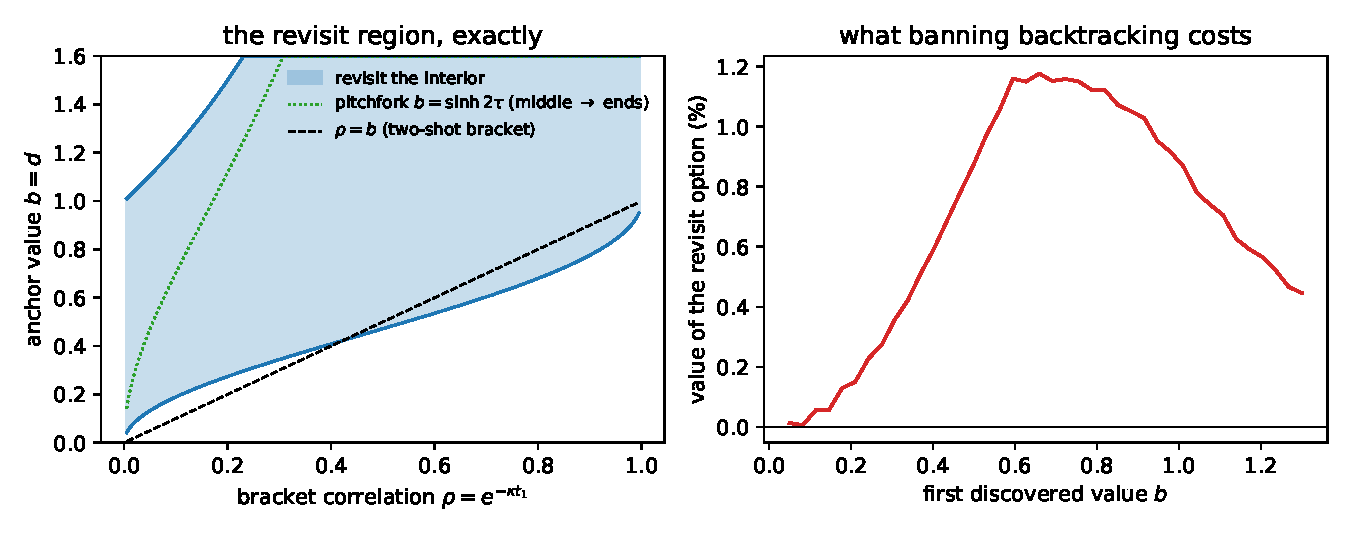
\includegraphics[width=\textwidth]{figures/phase.pdf}
\caption{Left: the exact symmetric revisit region \eqref{eq:region}
in the plane of bracket correlation $\rho$ and anchor value $b=d$,
bounded below by the quadratic root $b_{-}$ and above by
$e^{2\Theta}$. The dotted curve is the pitchfork $b=\sinh 2\tau$:
below it the optimal interior point is the bracket middle, above it
the mirror pair \eqref{eq:offmid} hugging the ends. The dashed line
is the two-shot bracket $\rho=b$, entering the region at
$b^{*}=0.4233$. Right: the value of the interior option --- the
percentage increase in expected payoff of the full three-shot optimum
over the best policy denied interior placements (it may still place
on either exterior ray) --- as a function of the first discovered
value $b$, with the bracket optimized in both cases.}
\label{fig:phase}
\end{figure}

\section{Beyond equal anchors}

For general $\left(b,d\right)$ the interior stationary points solve
the quartic
\begin{equation}\label{eq:quartic}
x^{4}-\left(b-\rho d\right)x^{3}+\rho\left(d-\rho b\right)x-\rho^{2}
\;=\;0,
\end{equation}
obtained by differentiating \eqref{eq:bridge}; its real roots in
$\left(\rho,1\right)$, compared against $\zeta(b)$ and $\zeta(d)$,
decide the move exactly and replace any grid. The symmetric window
does not extend indefinitely in $d$. At $b=\tfrac12$,
$\rho=\tfrac12$, the interior wins precisely for
$d\in\left(\approx 0.4715,\,1\right)$: below, the ray past the better end
wins; at $d=1$ every strictly interior point loses, by the identity
\begin{equation}
L(x)-1 \;=\;
-\frac{\left(2x-1\right)^{2}\left(x^{2}+x+1\right)}{6x^{2}}
\;<\;0, \qquad \tfrac12<x<1,
\end{equation}
and for $d\ge 1$ staying at the second anchor is optimal, since
$d$'s coefficient in the bridge mean is below one and raising $d$
only widens the loss. Symmetric dominance is a window, not a half-line.

\section{The three-shot policy, computed}

Writing $V\left(b,d,\rho\right)$ for the best of $\zeta(b)$,
$\zeta(d)$ and the interior optimum (via \eqref{eq:quartic}), the
three-shot value of a bracket $\rho$ is
$\log\E_d\!\left[e^{V\left(b,d,\rho\right)}\right]$ with
$d\sim N\!\left(b\rho,1-\rho^{2}\right)$, computed by adaptive
quadrature and optimized over $\rho$. The comparison policy denies interior placement but keeps both
exterior rays. It is not a ban on reversing direction.

\begin{table}[t]
\centering
\begin{tabular}{rcccc}
\toprule
$b$ & optimal $\rho$ & value & value, interior excluded & interior worth \\
\midrule
$0.1$ & $0.053$ & $0.8396$ & $0.8393$ & $0.03\%$ \\
$0.3$ & $0.167$ & $0.8723$ & $0.8692$ & $0.31\%$ \\
$0.5$ & $0.289$ & $0.9386$ & $0.9314$ & $0.73\%$ \\
$0.7$ & $0.402$ & $1.0375$ & $1.0271$ & $1.05\%$ \\
$0.83$ & $0.469$ & $1.1183$ & $1.1072$ & $1.12\%$ \\
$0.9$ & $0.502$ & $1.1670$ & $1.1562$ & $1.09\%$ \\
$1.2$ & $0.622$ & $1.4059$ & $1.3991$ & $0.68\%$ \\
\bottomrule
\end{tabular}
\caption{The three-shot game: optimal bracket correlation, log-value,
the log-value with interior placement excluded (exterior rays in both
directions permitted), and the percentage the interior option adds to
expected payoff. Adaptive quadrature over the second value $d$;
interior optima exact via the stationarity quartic
\eqref{eq:quartic}. For $b<0$ the optimal bracket correlation tends
to zero and the limiting log-value is exactly
$\tfrac12+\log\!\left(1+1/\sqrt{2\pi}\right)=0.8357\ldots$}
\label{tab:threeshot}
\end{table}

Three observations, all in Table~\ref{tab:threeshot} and
Figure~\ref{fig:phase}. First, a below-median start still means
flight, and the interior option is then worthless. Second, the
three-shot bracket is wider than the two-shot step, but most of the
widening is \emph{not} bought by the interior option: at $b=0.5$ the
two-shot policy steps to $\rho=0.5$, excluding interior placement
already widens the optimum to $\rho=0.323$, and admitting it widens
further to $\rho=0.289$. The extra evaluation and the choice it
enables account for most of the stretch; the interior option adds a
further, smaller pull. Third, the interior option's worth peaks near
$1.1\%$ of expected value around $b\approx 0.83$ and vanishes at both
extremes. Excluding interior placement is thus cheap by value; it is
the prescription that errs, and for equal anchors it errs exactly on
the revisit window \eqref{eq:region} --- high, but below the ceiling
$e^{2\Theta}$ above which both policies stay. For unequal
observations the erring region is a joint condition on
$\left(b,d,\rho\right)$, decided by the quartic of
Section~6, not membership of each value separately: at
$\rho=\tfrac12$, $b=\tfrac12$, $d=2$, both values lie in the
symmetric window, yet staying at the second anchor is optimal and
the exclusion costs nothing.

\section{The landscape premise on real measurements}\label{sec:wifi}

Whether real search fields look like exponentiated OU paths is
measurable. We use the WiFi positioning dataset of Feng, Nguyen and
Luo (2024): a university floor of $92\times 15$ meters on a
$0.6$-meter grid, 642 reference points, 13 access points, 120
repeated measurements per point over three days, released CC~BY.
Received power is a search field in the paper's literal sense: a
deployment seeks the location where signal is strongest, and the
landscape is rugged for physical reasons.

For each location and access point we form the mean linear power
over the repeats and take its logarithm, then remove an AP-specific
log-distance path-loss trend with the access-point position fitted.
The 4{,}235 surviving location--AP pairs form 50 corridor traces of
fifteen or more consecutive grid points. The residuals are close to
Gaussian (skewness $0.008$, excess kurtosis $0.05$), and their
pooled spatial correlation along corridors is exponential with
length $6.6$ meters and $R^2=0.98$ (Figure~\ref{fig:wifi}), the
form proposed for shadow fading by Gudmundson (1991) and standard in
radio engineering since. Roughly half the variance is a short-scale
component below the grid resolution: the surface is the paper's
curve plus fine gravel, and the replay below scores against the
surface as measured.

\begin{figure}[t]
\centering
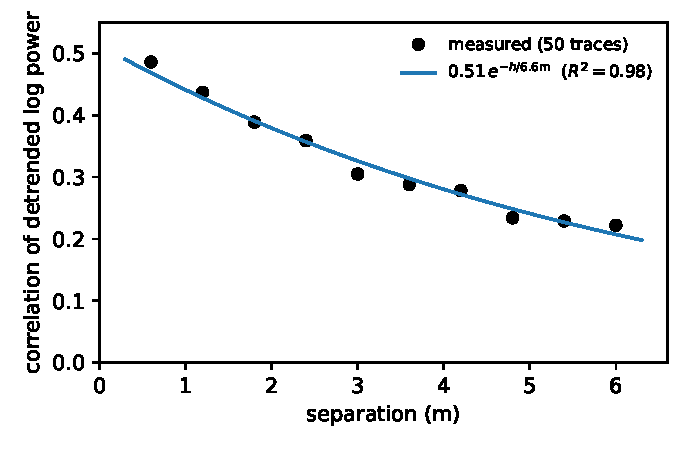
\includegraphics[width=0.6\textwidth]{figures/wifi_corr.pdf}
\caption{Pooled correlation of detrended log mean power along 50
corridor traces of the Feng et al.\ dataset, with the fitted
exponential. The landscape premise, measured.}
\label{fig:wifi}
\end{figure}

A trace-split replay makes the regime point concrete. The model is
fitted on half the traces; on each held-out trace a random
incumbent's value is revealed, one further measurement is placed by
each policy, and a deployment is committed and scored at the
measured surface. With correlation length near eleven grid units on
traces of fifteen to ninety-two, far probes are nearly fresh draws,
and the leading policies are the far-probing ones: probing the far
end gains $70\%$ of linear payoff over incumbent reuse and an
empirical knowledge gradient $63\%$, against $33\%$ for the
three-shot rule probing at the two-shot step. The exact formulas
predict this ordering: at bracket correlation $\rho$ the interior
option's premium is
$\tfrac12(e^{2\Theta}-1)(1-b^{2}e^{-2\Theta})\approx\rho(1-b^{2})$,
first order in $\rho$, while the fresh-draw variance bonus is order
one. The revisit machinery governs the opposite regime, search at
steps within a correlation length; adjacent grid points here sit at
$\rho=0.91$. Where a firm's feasible pivots are local, the phase
diagram is the operative map; where they are global, measure far
and take the best. The replay is a first pass: conditioning the
comparison on the phase-diagram region of each episode, and
per-trace intercepts in the fitted model, are the natural
refinements.

\section{Discussion}

Two distinct comparisons should not be merged. Against a \emph{visited} point of
matching conditional mean, any unvisited location wins by Jensen
alone: it carries variance, the known value carries none. Between two
\emph{unvisited} rivals of matching mean, an interior point and its
constructed exterior counterpart, Theorem~\ref{thm:dominance}
gives the constant variance ratio $e^{2\Theta}$. Neither comparison guarantees that a matched-mean unvisited point
exists when the observed value is high. Mean reversion caps the conditional
mean of every unvisited point, and above $b=e^{2\Theta}$ the cap
binds: the optimal final location is one already seen, and the grass,
there, is provably not greener. Below the cap the analysis locates the greenest patch: past the
better end on bad news, in whichever direction that end lies; between
the anchors on good news, at the middle for moderate anchors and
hugging an end beyond the pitchfork.

A caution about the word exploration. With one evaluation remaining
there is nothing to explore: no discovery at the final point can
inform a later choice. The last move is pure placement. The preference for uncertain
locations comes from Jensen's inequality, not from any value of
information.
Exploration proper enters only with more shots remaining. The natural conjecture from this endgame is a two-phase $k$-shot
policy: step out past the running best while values climb, then
refine between the two best once a good region is bracketed, with the
pitchfork inherited by the refinement phase. There is no irreversible
switch, since an adverse interior observation can make leaving
attractive again. The bridge formulas make each
policy evaluation cheap; the search over adaptive policies that a
$k$-shot dynamic program requires remains to be analyzed, and we make
no claim that it is small.

The problem solved here is terminal placement: the payoff is the
value at the final location, not the running maximum of the path.
Section~2 locates it in the literature; the short version is that
the tradition's exact objects are thresholds in
$\sigma^{2}/|\mu|$ on drifting Brownian paths with endogenous
evaluations and flow payoffs, and the fixed-budget, terminal-payoff,
mean-reverting combination, with its phase diagram, constant
amplification $e^{2\Theta}$, and constrained parabola
\eqref{eq:parabola}, is new.

\subsection*{Reproducibility}

All numbers and the figure are produced by \texttt{numerics2.py}
alongside this source; the review-driven identities (the constant
variance ratio, the $d=1$ factorization, the stationarity quartic,
the exact flee limit) are independently checked in
\texttt{verify/check\_review.py}, and the earlier counterexample
machinery lives in \texttt{verify/check\_inside.py} and
\texttt{verify/check\_middle.py}, all in the
\href{https://github.com/microprediction/browniansearch}{browniansearch}
repository.

\begin{thebibliography}{9}

\bibitem{callander2011}
S.~Callander.
Searching for good policies.
\emph{American Political Science Review}, 105(4):643--662, 2011.

\bibitem{callander2011b}
S.~Callander.
Searching and learning by trial and error.
\emph{American Economic Review}, 101(6):2277--2308, 2011.

\bibitem{bardhicallander2026}
A.~Bardhi and S.~Callander.
Learning in a correlated world.
\emph{Annual Review of Economics}, forthcoming.

\bibitem{bardhi2024}
A.~Bardhi.
Attributes: selective learning and influence.
\emph{Econometrica}, 92(2):311--353, 2024.

\bibitem{urgunyariv2025}
C.~Urgun and L.~Yariv.
Contiguous search: exploration and ambition on uncharted terrain.
\emph{Journal of Political Economy}, 133, 2025.

\bibitem{wong2025}
Y.~F. Wong.
Forward-looking experimentation of correlated alternatives.
\emph{Theoretical Economics}, 20, 2025.

\bibitem{callander2008}
S.~Callander.
A theory of policy expertise.
\emph{Quarterly Journal of Political Science}, 3(2):123--140, 2008.

\bibitem{callanderhummel2014}
S.~Callander and P.~Hummel.
Preemptive policy experimentation.
\emph{Econometrica}, 82(4):1509--1528, 2014.

\bibitem{callanderclark2017}
S.~Callander and T.~S. Clark.
Precedent and doctrine in a complicated world.
\emph{American Political Science Review}, 111(1):184--203, 2017.

\bibitem{callandermatouschek2019}
S.~Callander and N.~Matouschek.
The risk of failure: trial and error learning and long-run
performance.
\emph{American Economic Journal: Microeconomics}, 11(1):44--78, 2019.

\bibitem{callandermccarty2024}
S.~Callander and N.~McCarty.
Agenda control under policy uncertainty.
\emph{American Journal of Political Science}, 68(1):210--226, 2024.

\bibitem{clm2025}
S.~Callander, N.~S. Lambert, and N.~Matouschek.
Innovation and competition on a rugged technological landscape.
\emph{American Economic Journal: Microeconomics}, forthcoming.

\bibitem{aybas2025}
Y.~C. Aybas and S.~Callander.
Cheap talk in complex environments.
Working paper, 2025.

\bibitem{ganz2020}
S.~C. Ganz.
Hyperopic search: organizations learning about managers learning
about strategies.
\emph{Organization Science}, 31(4):821--838, 2020.

\bibitem{garfagnini2016}
U.~Garfagnini and B.~Strulovici.
Social experimentation with interdependent and expanding
technologies.
\emph{Review of Economic Studies}, 83(4):1579--1613, 2016.

\bibitem{cetemen2023}
D.~Cetemen, C.~Urgun, and L.~Yariv.
Collective progress: dynamics of exit waves.
\emph{Journal of Political Economy}, 131(9):2402--2450, 2023.

\bibitem{carnehl2025}
C.~Carnehl and J.~Schneider.
A quest for knowledge.
\emph{Econometrica}, 93(2):623--659, 2025.

\bibitem{hodgson2025}
C.~Hodgson and G.~Lewis.
You can lead a horse to water: spatial learning and path dependence
in consumer search.
\emph{Econometrica}, 93(4):1299--1332, 2025.

\bibitem{glick2015}
D.~Glick and C.~D. Myers.
Learning from others: an experimental test of Brownian motion
uncertainty models.
\emph{Journal of Theoretical Politics}, 27(4):588--612, 2015.

\bibitem{malladi2025}
S.~Malladi.
Searching in the dark and learning where to look.
Working paper, 2025.

\bibitem{banchio2025}
M.~Banchio and S.~Malladi.
Rediscovery.
Working paper, arXiv:2504.19761, 2025.

\bibitem{grosse2023}
J.~Grosse, C.~Zhang, and P.~Hennig.
Optimistic optimization of Gaussian process samples.
\emph{Transactions on Machine Learning Research}, 2023.

\bibitem{feng2024}
X.~Feng, K.~A. Nguyen, and Z.~Luo.
WiFi RTT RSS dataset for indoor positioning.
Zenodo, 2024. doi:10.5281/zenodo.11558192.

\bibitem{gudmundson1991}
M.~Gudmundson.
Correlation model for shadow fading in mobile radio systems.
\emph{Electronics Letters}, 27(23):2145--2146, 1991.

\bibitem{ries2011}
E.~Ries.
\emph{The Lean Startup}.
Crown Business, New York, 2011.

\bibitem{camuffo2020}
A.~Camuffo, A.~Cordova, A.~Gambardella, and C.~Spina.
A scientific approach to entrepreneurial decision making: evidence
from a randomized control trial.
\emph{Management Science}, 66(2):564--586, 2020.

\bibitem{camuffo2024}
A.~Camuffo, A.~Gambardella, D.~Messinese, E.~Novelli, E.~Paolucci,
and C.~Spina.
A scientific approach to entrepreneurial decision making: large
scale replication and extension.
\emph{Strategic Management Journal}, 45(6):1209--1237, 2024.

\bibitem{baumann2019}
O.~Baumann, J.~Schmidt, and N.~Stieglitz.
Effective search in rugged performance landscapes: a review and outlook.
\emph{Journal of Management}, 45(1):285--318, 2019.

\bibitem{grill2018}
J.-B. Grill, M.~Valko, and R.~Munos.
Optimistic optimization of a Brownian.
In \emph{Advances in Neural Information Processing Systems~31}, 2018.

\bibitem{calvin1997}
J.~M. Calvin.
Average performance of a class of adaptive algorithms for global
optimization.
\emph{Annals of Applied Probability}, 7(3):711--730, 1997.

\bibitem{alabert2018}
A.~Alabert and R.~Caballero.
On the minimum of a conditioned Brownian bridge.
\emph{Stochastic Models}, 34(3):269--291, 2018.

\bibitem{agrawal1995}
R.~Agrawal.
The continuum-armed bandit problem.
\emph{SIAM Journal on Control and Optimization}, 33(6):1926--1951, 1995.

\end{thebibliography}

\end{document}
